\documentclass{IEEEtran}
\usepackage{color}
\usepackage{amsmath}
\usepackage{booktabs}
\usepackage{graphicx}
\usepackage{algorithm2e}

% i have equations defined in a .tex file, which is used by this report, and the presentation. the
% presentation makes use of beamer's \alert{} macro. but here, \alert{} is not defined. define it so
% that it just passes through the argument without any additional formatting.
\newcommand{\alert}[1]{#1}
\renewcommand{\vec}[1]{\mathbf{#1}}
\newcommand{\half}{\frac{1}{2}}
\newcommand{\loss}{\Delta\left(\vec{y}, \vec{y}_i\right)}

% Traditional SVM Equation
\def\svmEquation
{
\begin{align}
    \min_\vec{w} & \half \vec{w} \cdot \vec{w} + C\sum_{i=1}^n\xi_i \\
    \text{s.t. } & \forall i \xi_i \ge 0 \nonumber \\
                 & \forall i y_i \left(\vec{w} \cdot \vec{x}_i + b\right) \ge 1 - \xi_i \nonumber
\end{align}
}

% Traditional SVM Dual
\def\traditionalDual
{
\begin{align}
    \max_\alpha & \sum_{i=1}^n \alpha_i - \half \sum_{i=1}^n \sum_{j=1}^n \alpha_i \alpha_j
    y_i y_j K\left(\vec{x}_i, \vec{x}_j\right) \\
    \text{s.t. } & \sum_{i=1}^n y_i \alpha_i = 0 \nonumber \\
    & 0 \le \alpha_i \le C \nonumber
\end{align}
}

% Fuzzy SVM Equation
\def\fuzzySvmEquation
{
\begin{align}
    \min_\vec{w} & \half \vec{w} \cdot \vec{w} + C\sum_{i=1}^n \alert{s_i} \xi_i \\
    \text{s.t. } & \forall i \xi_i \ge 0 \nonumber \\
                 & \forall i y_i \left(\vec{w} \cdot \vec{x}_i + b\right) \ge 1 - \xi_i \nonumber
\end{align}
}

% Fuzzy SVM Dual
\def\fuzzyDual
{
\begin{align}
    \max_\alpha & \sum_{i=1}^n \alpha_i - \half \sum_{i=1}^n \sum_{j=1}^n \alpha_i \alpha_j
    y_i y_j K\left(\vec{x}_i, \vec{x}_j\right) \\
    \text{s.t. } & \sum_{i=1}^n y_i \alpha_i = 0 \nonumber \\
    & 0 \le \alpha_i \le \alert{s_i} C \nonumber
\end{align}
}


\begin{document}
\title{Fuzzy Structured Output Tracking with Kernels}
\author{Brendan Robeson}
\date{\today}
\maketitle

\begin{abstract} %start_fold_1
    Tracking an object in a video or image stream has many practical applications, from enhancing a
    sports video broadcast, to military surveillance and reconnaissance. A common approach to the
    problem of object tracking is tracking-by-detection. This involves the use of pattern
    recognition techniques to classify samples of the current frame as the target object, or not the
    target object. Such samples frequently contain only some subset of the target object features.
    In this paper, I build on a fairly robust tracking algorithm, introducing fuzzy logic to the
    employed SVM.
\end{abstract}

\section{Introduction} %start_fold_1
Object tracking in video is a challenging problem in the area of computer vision. Several tracking
obstacles can arise in video sequences which can confuse a tracker. These include: occlusion of the
target object, change in the target object size and shape, change in lighting, and a shaky camera to
name a few. In 2014, a review of several tracking algorithms \cite{6671560} identified which
algorithms were best with respect to specific tracking challenges, and which algorithms were best
overall. Struck \cite{6126251} was rated as the best overall, though is not perfect \cite{6671560}.

Struck provides an good option for tracking research. It is an excellent tracker to start with, but
has room for improvement. In this paper, I propose an alternative, Fuzzy Struck. It is a merging of
Struck, with fuzzy SVM. Struck samples around the target object to update its SVM \cite{6126251}. It
does not consider that such samples contain only a portion of the target features. Figure
\ref{fig:surfer} shows an example of this. In this figure, the red box outlines the surfer to be
tracked through the video. The blue box outlines a sample extracted from the frame, which is used to
update the tracker. The sample will contain, at most, 25\% of the features contained in target
bounding box.

The rest of the introduction provides a review of fuzzy SVM and Struck. In section 2, I describe the
Fuzzy Struck algorithm. In section 3, I detail the experiments uses to compare Fuzzy Struck with
Struck, and analyze the results. Finally, I conclude with further research areas.

\subsection{Fuzzy SVM} %start_fold_2
Fuzzy SVM \cite{991432} reformulates the SVM to incorporate fuzzy membership data for the classes. The
traditional SVM formula
\svmEquation
becomes
\fuzzySvmEquation
where \(s_i\) is the fuzzy membership.

The dual problem is then
\fuzzyDual

Fuzzy membership is calculated by a function \(s_i = f(\cdot)\). The exact function depends on the
classification problem to be solved, but should satisfy \(0 \le \theta \le f(\cdot) \le 1\).
\(\theta\) is a predefined lower bound, also dependent on the classification problem.

% put this here, so it's not in the first column of the first page
\begin{figure}
    \centering
    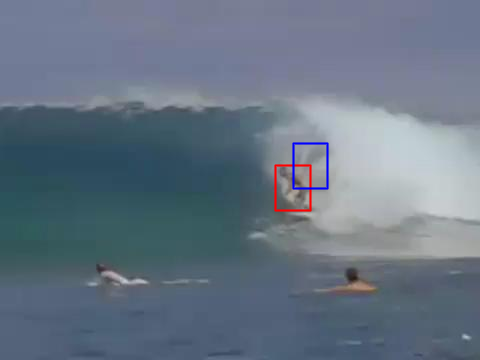
\includegraphics[width=2.5in]{surfer_sample}
    \caption{The red box outlines the surfer to track. The blue box shows a sample used for updating
    the tracker. The sample contains no more than 25\% of the target.}
    \label{fig:surfer}
\end{figure}

\subsection{Struck} %start_fold_2
Struck \cite{6126251} is an adaptive tracking algorithm. For frame \(n\), the algorithm samples
radially around the object location in frame \(n-1\). A structured output SVM is used to predict the
location of the object in frame \(n\). Once the object is found, the SVM is updated; thus it learns as
the object is tracked in the sequence.

A traditional SVM takes, as training input, data of the form \((\vec{x}, y)\), where
\(\vec{x}\) is a feature vector, and \(y \in \{-1, +1\}\) is a class label. The training input of
a structured output SVM takes the form \((\vec{x}, \vec{y})\). As in a traditional SVM,
\(\vec{x}\) is a feature vector. In this case, however, \(\vec{y} \in \mathcal{Y}\) is a prediction
function. In Struck, the prediction function is a transformation from the object location, to the
sample location.

The SVM equation used in Struck is
\struckEquation

Optimizing in terms of \(\alpha\) leads to
\struckDualAlpha

According to \cite{Bordes:2007:SMS:1273496.1273508}, \eqref{eq:struck_dual_alpha} can be simplified
by reparametrizing in terms of \(\beta\).
\struckDualBeta

This equation can be solved by the sequential minimal optimization algorithm
\cite{sequential-minimal-optimization-a-fast-algorithm-for-training-support-vector-machines}, shown
in the following algorithm.

\struckSmo

Struck also incorporates a budget for the support vectors \cite{6126251}. This prevents the
algorithm from slowing down too much, and limits overfitting of the SVM. Struck selects the vectors
to remove based on minimum change in the SVM's weight vector. This change is given by
\struckWeightChange

%Discriminant function
%
%\begin{displaymath}
%    F(\vec{x}, \vec{y}) = \sum_{i,\vec{\bar{y}}} \beta_i^\vec{\bar{y}}
%    \vec{\Phi}\left(\vec{x}_i, \vec{\bar{y}}\right) \cdot \vec{\Phi}\left(\vec{x},
%    \vec{y}\right)
%\end{displaymath}
%
%Gradient
%\begin{align}
%    g_i\left(\vec{y}\right) &= - \loss - \sum_{j,\vec{\bar{y}}} \beta_j^\vec{\bar{y}}
%    \vec{\Phi}\left(\vec{x}_i, \vec{y}\right) \cdot \vec{\Phi}\left(\vec{x}_j,
%    \vec{y}\right) \\
%    &= - \loss - F\left(\vec{x}_i, \vec{y}\right) \nonumber
%\end{align}

\section{Fuzzy Struck} %start_fold_1
\subsection{Fuzzy Structured Output SVM} %start_fold_2
Fuzzy Struck combines the fuzzy SVM with the structured output SVM of Struck. Incorporating fuzzy
membership into Struck results in the following SVM equation
\fuzzyStruckEquation

The dual optimization is then given by
\fuzzyStruckDualAlpha

As in \cite{sequential-minimal-optimization-a-fast-algorithm-for-training-support-vector-machines}
and \cite{6126251}, this can be reparametrized as
\fuzzyStruckDualBeta

Note that the fuzzy membership, \(s_i\), influences the constraints on \(\alpha\) and, in turn,
\(\beta\). This, then, alters the sequential minimal optimization as shown in the following
algorithm:

\fuzzyStruckSmo

\subsection{Budget Maintenance} %start_fold_2
Fuzzy Struck also incorporates the fuzzy membership during support vector budget maintenance.
Whereas Struck removes the vectors with minimal influence on the SVM weights, Fuzzy Struck removes
the vectors with minimum membership. Notice that in \eqref{eq:struck_weights}, two factors can
influence the change in weights: the \(\beta\) value, and the sum of the dot products. In Fuzzy
Struck, the sum of the dot products is removed from consideration for budget maintenance. The fuzzy
membership only influences \(\beta\), not the dot products.

\subsection{Fuzzy Membership} %start_fold_2
For F-Struck, the fuzzy membership function is defined as a function of bounding box overlap. In
this context, a sample bounding box with high overlap will contain more of the target; low overlap
will contain less of the target.

\begin{displaymath}
    s_i = f\left(b, b_i\right) = \frac{A(b \cap b_i)}{A(b \cup b_i)}
\end{displaymath}

where \(b\) defines the target bounding box, and \(b_i\) defines the sample bounding box, and
\(A(x)\) is the area of \(x\). If the two bounding boxes do not intersect, then \(A\left(b \cap
b_i\right) = 0\), and thus \(s_i = 0\). If the bounding boxes coincide exactly,
\(A\left(b \cap b_i\right) = A\left(b \cup b_i\right)\), and \(s_i = 1\).

\section{Experiments} %start_fold_1
A comparison between the original Struck and Fuzzy Struck shows the effect of fuzzy
membership. The source code for Struck is available online.\footnote{https://github.com/samhare/struck}
This was used to generate experimental results for Struck. It was also the basis for Fuzzy Struck;
Fuzzy Struck was created by modifying the Struck source code.

The set up for the experiments was as follows: Haar features were extracted from the frame samples,
and input to the SVM. A Gaussian kernel function was used, with \(\sigma = 0.2\). The search radius
was fixed at 30 pixels, the SVM budget at 100 support vectors, and the random seed at 0. Most of the
these settings are the same as reported in \cite{6126251}. The exception is the random seed, which
was not reported. The random seed of 0 is the value in the default configuration file included with
the Struck source code.

The experiments were run for integer values of C, from 1 to 100. Roughly half the values of C
resulted in better performance in Struck, while the remaining values of C resulted in better
performance for Fuzzy Struck. This will be discussed more in the conclusion below.

The algorithms were run for twelve publicly available video
sequences.\footnote{http://vision.ucsd.edu/~bbabenko/project\_miltrack.html} Eight of these
sequences were reported in \cite{6126251}; the remaining four were not reported, for unknown
reasons. Measuring the algorithms' results was done via bounding box overlap. For each frame with
a ground truth bounding box, the algorithm output was compared with the ground truth. Two bounding
boxes which overlap exactly will have an overlap value of 1. If the two boxes do not overlap at all,
the value will be 0. For each sequence, the average bounding box overlap was calculated. Table
\ref{tab:results} shows the results for \(C = 100\). Bold values indicate the better result.

\begin{center}
%\begin{tabular}{l r r r}
%    \toprule
%    Sequence & Struck & \(s_{min}\) removal & no \(s_i = 0\) \\
%    \midrule
%    girl     &         0.681729  & \textbf{0.681821} & \textbf{0.681821} \\
%    surfer   &         0.787232  &         0.787232  & \textbf{0.811688} \\
%    tiger1   &         0.674713  &         0.651670  & \textbf{0.746060} \\
%    tiger2   &         0.667268  &         0.509582  & \textbf{0.679176} \\
%    twinings &         0.903097  & \textbf{0.931334} & \textbf{0.907482} \\
%    dollar   &         0.765203  &         0.765203  &         0.765203  \\
%    faceocc  &         0.853354  &         0.853354  &         0.853354  \\
%    cliffbar & \textbf{0.894553} &         0.890760  &         0.717940  \\
%    coke11   & \textbf{0.883395} &         0.882497  &         0.841359  \\
%    david    & \textbf{0.800847} &         0.434802  &         0.434802  \\
%    faceocc2 & \textbf{0.790128} &         0.789270  &         0.789270  \\
%    sylv     & \textbf{0.861525} &         0.857138  &         0.858211  \\
%    \bottomrule
%\end{tabular}

\begin{tabular}{l r r}
    \toprule
    Sequence & Struck & Fuzzy Struck \\
    \midrule
    girl     &         0.681729  & \textbf{0.681821} \\
    surfer   &         0.787232  & \textbf{0.811688} \\
    tiger1   &         0.674713  & \textbf{0.746060} \\
    tiger2   &         0.667268  & \textbf{0.679176} \\
    twinings &         0.903097  & \textbf{0.907482} \\
    dollar   &         0.765203  &         0.765203  \\
    faceocc  &         0.853354  &         0.853354  \\
    cliffbar & \textbf{0.894553} &         0.717940  \\
    coke11   & \textbf{0.883395} &         0.841359  \\
    david    & \textbf{0.800847} &         0.434802  \\
    faceocc2 & \textbf{0.790128} &         0.789270  \\
    sylv     & \textbf{0.861525} &         0.858211  \\
    \bottomrule
\end{tabular}
\end{center}


Figures \ref{fig:sylv} and \ref{fig:faceocc2} show sample frames from two sequences with tracking
results. Figure \ref{fig:sylv} is from the Sylv sequence. Notice that the Fuzzy Struck bounding box
is more closely aligned with the ground truth than is the Struck bounding box. The opposite is true
in Figure \ref{fig:faceocc2}, from the Faceocc2 sequence.

\begin{figure}[!t]
    \centering
    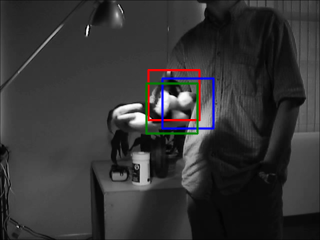
\includegraphics[width=2.5in]{sylv.png}
    \caption{Frame from the Sylv sequence with target bounding boxes. Red is the ground truth, blue
    is Struck, green is Fuzzy Struck.}
    \label{fig:sylv}
\end{figure}

\begin{figure}[!t]
    \centering
    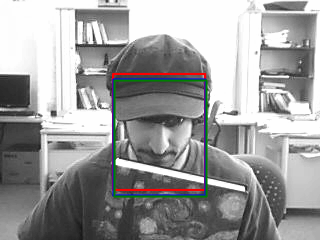
\includegraphics[width=2.5in]{faceocc2.png}
    \caption{Frame from the Faceocc2 sequence with target bounding boxes. Red is the ground truth,
    blue is Struck, green is Fuzzy Struck.}
    \label{fig:faceocc2}
\end{figure}

There are a few items of note with these results. First, the value of C in the SVM has a significant
influence on the tracker results. Further, there is no clear pattern or cut off for the value of C.
The values of C for which Fuzzy Struck did better than Struck were scattered within the set of C.

Second, introduction of fuzzy membership has, in general, improved tracking for some sequences, but
made it worse in others. The dominant factor appears to be selection of support vectors for removal
during budget maintenance. Removing that aspect of Fuzzy Struck reverses some, but not all, of the
results. That is, reverting the support vector remove choice can change which algorithm is the
better tracker for some sequences. This is hypothesized to be due to the nature of dot products. The
dot product of two vectors is proportional to the cosine of the angle between those two vectors. The
minimum cosine occurs when two vectors are opposite in direction. This factor is not considered in
Fuzzy Struck.

\section{Conclusion} %start_fold_1
In this paper, I presented a modification to Struck, incorporating fuzzy membership into the
algorithm. For most sequences, this modification improves the tracking results. Degradation of
tracking results for other sequences presents further research areas. Selection of an optimal value
of C is one such question. Another is the best method of selecting support vectors for removal when
on a budget. Finally, how selection and updating of fuzzy membership influence the tracker? In this
paper, fuzzy membership is a function of bounding box overlap. Other possible functions include
time or target velocity.

%\section{Notes} %start_fold_1
%\begin{align*}
%    \min_\vec{w} & \half \vec{w} \cdot \vec{w} + C \sum_{i=1}^n \textcolor{red}{s_i} \xi_i \\
%    \text{s.t. } & \textcolor{red}{s_i} \xi_i \ge 0 \\
%    & \vec{w} \cdot \delta \vec{\Phi}_i(y) \ge \loss - \textcolor{red}{s_i} \xi_i
%\end{align*}
%
%\begin{align*}
%    \max_\alpha & \sum_i \loss \alpha_i^y - \half \sum_{i,j} \alpha_i^y
%    \alpha_j^{\bar{y}} \delta \vec{\Phi}_i(y) \cdot \delta \vec{\Phi}(\bar{y}) \\
%    \text{s.t. } & \forall y \ne y_i : \alpha_i^y \ge 0 \\
%    & \sum_{y \ne y_i} \alpha_i^y \le C
%\end{align*}
%
%\newpage
%
%\subsection{LaGrange} %start_fold_2
%\begin{align}
%    f &= \half \vec{w} \cdot \vec{w} + C \sum_{i=1}^n \textcolor{red}{s_i} \xi_i \\
%    g_1 &= \xi_i \ge 0 \\
%    g_2 &= \vec{w} \cdot \delta \vec{\Phi}\left(y_i\right) + \textcolor{red}{s_i} \xi_i - \loss \ge 0 \\
%    &= \vec{w} \cdot \left(\vec{\Phi}\left(y_i\right) - \vec{\Phi}(y)\right) + \textcolor{red}{s_i} \xi_i
%    - \loss \ge 0 \nonumber
%\end{align}
%\begin{align}
%    J &= f - \alpha g_1 - \beta g_2 \\
%    J &= \half \vec{w} \cdot \vec{w} + C \sum_{i=1}^n \textcolor{red}{s_i} \xi_i -
%        \sum_i \alpha_i \xi_i \nonumber \\ & -
%        \sum_i \beta_i \left[\vec{w} \cdot \delta \vec{\Phi}\left(y_i\right) + \textcolor{red}{s_i} \xi_i
%        - \loss\right] \nonumber \\
%    J &= \half \vec{w} \cdot \vec{w} + C \sum_{i=1}^n \textcolor{red}{s_i} \xi_i -
%        \sum_i \alpha_i \xi_i \nonumber \\ & -
%        \sum_i \left[ \beta_i \vec{w} \cdot \delta \vec{\Phi}\left(y_i\right) + \beta_i
%        \textcolor{red}{s_i} \xi_i - \beta_i \loss\right] \nonumber \nonumber
%\end{align}
%
%% derivative with respect to w
%\begin{align}
%    \frac{\partial J}{\partial \vec{w}} = 0 &= \vec{w} - \sum_i \beta_i \delta \vec{\Phi}\left(y_i\right) \\
%    \vec{w} &= \sum_i \beta_i \delta \vec{\Phi}\left(y_i\right) \nonumber
%\end{align}
%
%% derivative with respect to ξ
%\begin{align}
%    \frac{\partial J}{\partial \xi_i} = 0 &= C \textcolor{red}{s_i} - \alpha_i - \beta_i \textcolor{red}{s_i}
%\end{align}

\bibliographystyle{IEEEtran} %start_fold_1
\bibliography{references}

\end{document}
